%; whizzy paragraph -pdf xpdf -latex ./whizzypdfptex.sh
%; whizzy-paragraph "^\\\\begin{frame}"
% latex beamer presentation.
% platex, latex-beamer $B$G%3%s%Q%$%k$9$k$3$H$rA[Dj!#(B 

%     Tokyo Debian Meeting resources
%     Copyright (C) 2009 Junichi Uekawa
%     Copyright (C) 2009 Nobuhiro Iwamatsu

%     This program is free software; you can redistribute it and/or modify
%     it under the terms of the GNU General Public License as published by
%     the Free Software Foundation; either version 2 of the License, or
%     (at your option) any later version.

%     This program is distributed in the hope that it will be useful,
%     but WITHOUT ANY WARRANTY; without even the implied warranty of
%     MERCHANTABILITY or FITNESS FOR A PARTICULAR PURPOSE.  See the
%     GNU General Public License for more details.

%     You should have received a copy of the GNU General Public License
%     along with this program; if not, write to the Free Software
%     Foundation, Inc., 51 Franklin St, Fifth Floor, Boston, MA  02110-1301 USA

\documentclass[cjk,dvipdfm,12pt]{beamer}
\usetheme{Tokyo}
\usepackage{monthlypresentation}

%  preview (shell-command (concat "evince " (replace-regexp-in-string "tex$" "pdf"(buffer-file-name)) "&"))
%  presentation (shell-command (concat "xpdf -fullscreen " (replace-regexp-in-string "tex$" "pdf"(buffer-file-name)) "&"))
%  presentation (shell-command (concat "evince " (replace-regexp-in-string "tex$" "pdf"(buffer-file-name)) "&"))
%  presentation (shell-command (concat "evince " (replace-regexp-in-string "tex$" "pdf"(buffer-file-name)) "&"))

%http://www.naney.org/diki/dk/hyperref.html
%$BF|K\8l(BEUC$B7O4D6-$N;~(B
\AtBeginDvi{\special{pdf:tounicode EUC-UCS2}}
%$B%7%U%H(BJIS$B7O4D6-$N;~(B
%\AtBeginDvi{\special{pdf:tounicode 90ms-RKSJ-UCS2}}

\title{Auto-builder $B%M%C%H%o!<%/(B}
\subtitle{$B;qNA(B}
\author{$B4d>>(B $B?.MN(B iwamatsu@debian.org\\IRC nick: iwamatsu}
\date{2009$BG/(B11$B7n(B14$BF|(B}
\logo{
\includegraphics[width=8cm]{image200607/openlogo-light.eps}}

%begin of commandline0
\newenvironment{commandline0}%
{\VerbatimEnvironment
  \begin{Sbox}\begin{minipage}{0.95\hsize}\begin{fontsize}{9}{9} \begin{BVerbatim}}%
{\end{BVerbatim}\end{fontsize}\end{minipage}\end{Sbox}
  \setlength{\fboxsep}{10pt}

\vspace{10pt}% skip before
\fcolorbox{dancerdarkblue}{dancerlightblue}{\TheSbox}

\vspace{6pt}% skip after
}
%end of commandline0

\begin{document}

\frame{\titlepage{}}

\begin{frame}{autobuilder $B%M%C%H%o!<%/$H$O(B}
\begin{itemize}
\item Debian Project $B$N=EMW$J%7%9%F%`$N0l$D(B
\item $B3F%"!<%-%F%/%A%cKh$K%Q%C%1!<%8$r<+F0E*$K%S%k%I$9$k!#(B
\end{itemize}
\end{frame}

\begin{frame}{Autobuilder $B%M%C%H%o!<%/$N%3%s%]!<%M%s%H(B}
\begin{itemize}
\item dak
\item quinn-diff
\item wanna-build
\item buildd
 
\begin{itemize}
\item buildd
\item buildd-mail
\item buildd-mail-wrapper
\item buildd-update-chroots
\item buildd-uploader
\item buildd-watcher
\end{itemize}

\item sbuild
\item schroot
\item porter
\item wanna-build $B%a%s%F%J(B
\end{itemize}

\end{frame}

\begin{frame}{$B3F%3%s%]!<%M%s%H$H$NO"7H(B}
\begin{center}
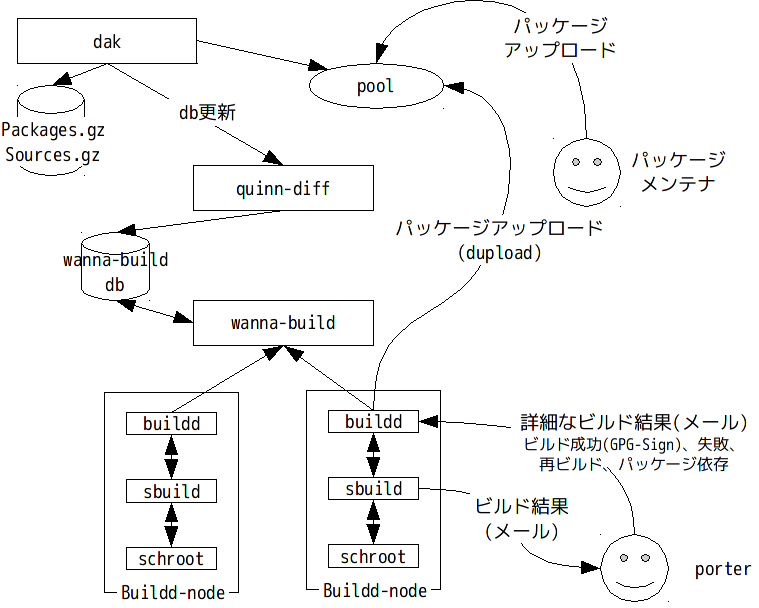
\includegraphics[width=1.1\hsize]{image200911/buildd-image00.png}
\end{center}
\end{frame}

\begin{frame}{$B%Q%C%1!<%8$N%9%F!<%?%9(B}
\begin{itemize}
\item BD-Uninstallable
\item Needs-Build 
\item Building 
\item Uploaded
\item Installed
\item Dep-Wait
\item Failed
\item Not-For-Us
\item Failed-Removed
\end{itemize}
\end{frame}

\begin{frame}{$B%9%F!<%?%9$N>uBVA+0\(B}
\begin{center}
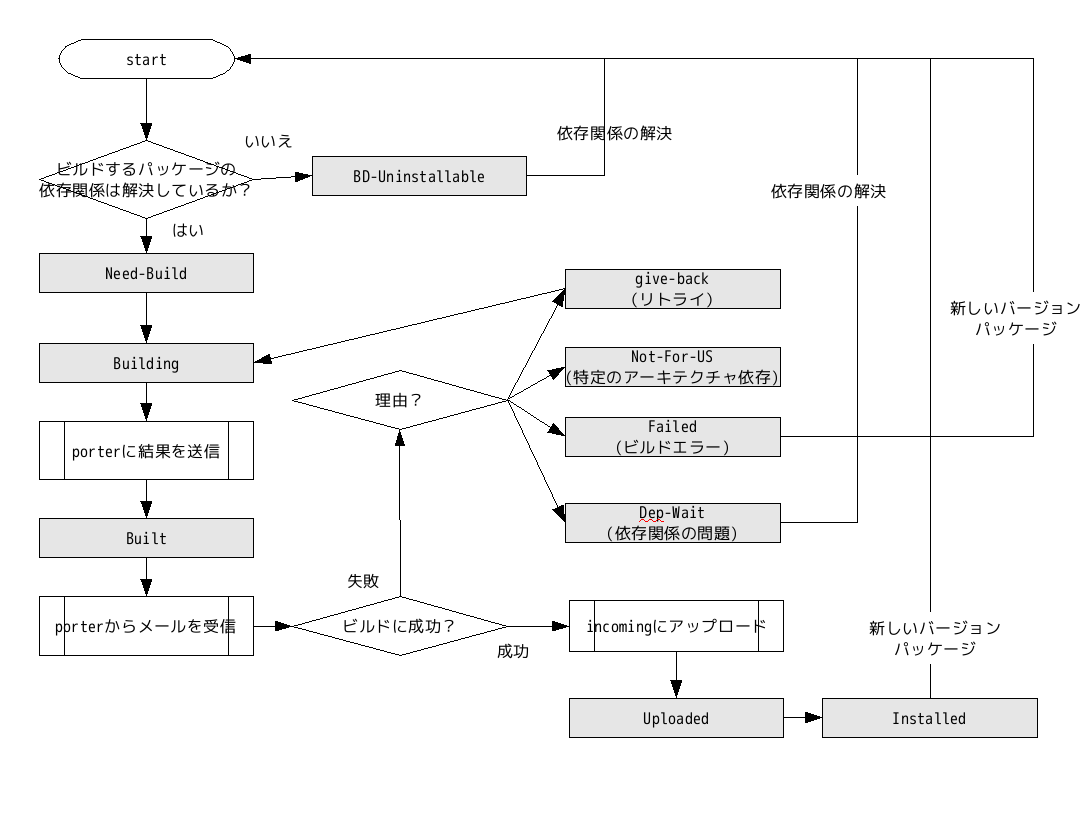
\includegraphics[width=0.9\hsize]{image200911/buildd-status.png}
\end{center}
\end{frame}

\begin{frame}{$B%Q%C%1!<%8%S%k%IM%@h=g0L(B}

$B%Q%C%1!<%8%S%k%I$NM%@h=g0L$,7h$^$C$F$$$k!#(B
\begin{enumerate}
\item $B%=!<%9%Q%C%1!<%8$N%W%i%$%*%j%F%#(B
\item $B%=!<%9%Q%C%1!<%8$N%;%/%7%g%s(B
\item $B%Q%C%1!<%8L>(BASCII $B=g(B
\item Need-Build $B$N%9%F!<%?%9$K$J$C$?=g(B 
\end{enumerate}

\end{frame}

\begin{frame}{$B?7$7$$%"!<%-%F%/%A%c$rDI2C$9$k(B}

\begin{itemize}
\item buildd.debian.ort $B$K$O$9$0$K$ODI2C$9$k$3$H$O$G$-$J$$(B
\item debian-ports.org
\item quinn-diff $B$H(B wanna-build $B%5!<%S%9$rDs6!(B
\item $B8=:_!"(Bhurd-1386, m68k, avr32, sh4 $B$,$3$N%5!<%S%9$rMxMQCf!#(B
\end{itemize}
\end{frame}



\begin{frame}[containsverbatim]{loop-depends $BBP1~(B}

\begin{enumerate}
\item loop-depends\\
$B%Q%C%1!<%8$,%k!<%W$7$F%S%k%I0MB8$7$F$$$k>uBV!#(B\\

\item $BNc(B
\begin{commandline}
- libgtk2-perl -> libpang-perl -> 
        libgtk2-perl -> libpang-perl -> .....
- cups -> avahi -> pygtk -> librsvg -> 
        libgsf -> gnome-vfs  -> gconf -> cups
\end{commandline}

\item $B=$@5J}K!$O7h$^$C$F$$$J$$(B
\item unreleased $B%G%#%9%H%j%S%e!<%7%g%s$rMxMQ$9$k(B

\end{enumerate}
\end{frame}


\begin{frame}{loop-depends $BBP1~(B}
\begin{center}
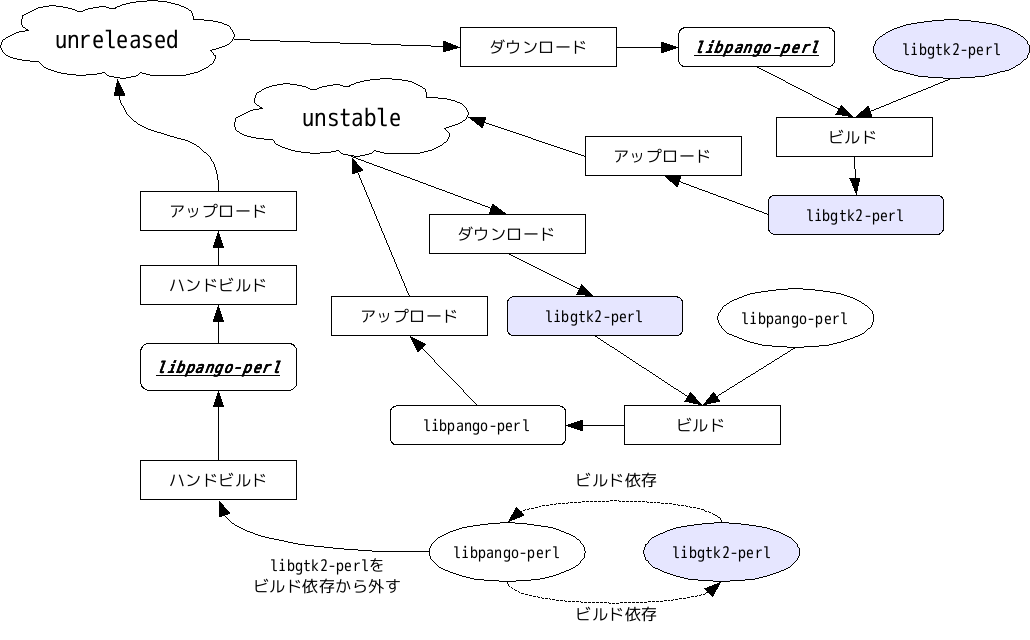
\includegraphics[width=1.1\hsize]{image200911/loop-dep-image.png}
\end{center}
\end{frame}

\begin{frame}{$B<ALd(B}
\begin{center}
\Huge{$B2?$+<ALd$O$"$j$^$9$+!)(B}
\end{center}
\end{frame}


\end{document}

;;; Local Variables: ***
;;; outline-regexp: "\\([ 	]*\\\\\\(documentstyle\\|documentclass\\|emtext\\|section\\|begin{frame}\\)\\*?[ 	]*[[{]\\|[]+\\)" ***
;;; End: ***
